\section{Existing methods}

\subsection{Machine learning methods} \label{dl_methods}
There are a variety of LLM (Large language model) architectures that were applied to the task of language modeling. One significant example is \texttt{LSTM} (Long short-term memory) model, that was introduced by \textcite{lstm_1997}. \texttt{LSTM} is a variation of \texttt{RNN} (Recurrent neural network), and it was widely applied to language modeling, including morphology modeling. Another more recent significant example is the transformer architecture presented by \textcite{transformer_2017}, off which two years later \texttt{BERT} (Bidirectional encoder representations from transformers) model was based \parencite{devlin_2019}. 

One of the biggest downsides of ML methods is that its quality depends on training data quantity, which makes it challenging to apply to low-resourse languages such as Shughni. However, with introduction of LLMs this problem was shown to be solvable, for example, as shown by developers of \texttt{UDify} model \parencite{kondratyuk_straka_model_2019}, which is a \texttt{BERT}-based model. In their work authors show, that their model pretrained on a large corpus of 104 languages can be fine-tuned on very little amounts of other languages' data and till show decent results. For an example, they report that for Belarusian, \texttt{UDify} model achieved $UFeats=89.36\%$ (accuracy of tagging Universal Features) after training on only 261 sentences from `Belarusian HSE' Universal Dependencies treebank \parencite[Table 7]{kondratyuk_straka_model_2019}.

However, working with LLM models is a highly resource-demanding task. The authors of \texttt{UDify} state, that the fine-tuning of their model for a new language would require at least 16 Gigabytes of RAM and at least 12 Gigabytes of GPU video memory, and the training process would take at least 20 days depending on the GPU model. While a deep learning approach would be interesting to explore, such computational resources are not available for this project. The neural approach is not the main target of this work and is not implemented. 

\subsection{Rule-based methods}
\subsubsection{Finite-state transducers}
The Rule-based approach historically is usually applied with the help of Finite-state transducers (FST), which is a variation of Finite-state machine, a mathematical abstract computational model. Following the terminology of Turing machines \parencite{Turing_1937}, a FST has two tapes: the input tape and the output tape. At any point it can read a next symbol from the input tape and then write a symbol to the output tape. Once a symbol was read from the input tape, it can not be read again, as the input tape shifts one symbol forward. \todo{Старайтесь ссылаться в тексте на любые рисунки и таблицы, которые Вы вставляете.}

\begin{figure}[!h]
    \centering
    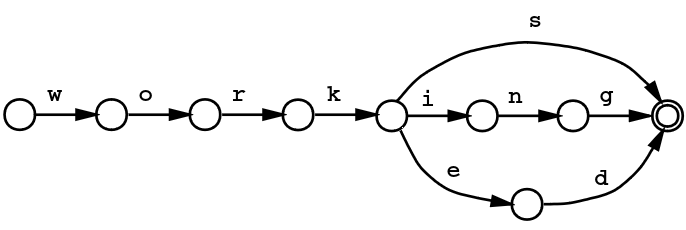
\includegraphics[scale=0.5]{\rootdir/img/transducer1.png}
    \caption{An example of FSA with a single initial state (most left node) and a single final state (most right node) for a language where only three words exist: \textit{works}, \textit{working} and \textit{worked}. The word \textit{worker}, for example will not be recognized as a valid word by this FSA, since there is no 'r' transition at state \textit{worke}. The only way from \textit{worke} state is via 'd' transition, which corresponds to the \textit{worked} word. \parencite{beesley_fst_2002}}
    \label{fig:fst1}
\end{figure}

\todo{У Вас здесь смешался в описании конечный автомат и трансдьюссер. Вы даже пишите recognize --- поведение конечных автоматов.}

The inner structure of FST can be illustrated as a directed graph with a set of all \textit{states} (represented by graph's nodes), a set of \textit{transitions} (represented by graph's edges), a set of \textit{initial states} (a subset of all the states, these are states where FST can start reading from the input tape) and a set of \textit{final states} (a subset of all the states, these are the states where FST can stop reading from the input tape). A simplified FST is shown on Figure \ref{fig:fst1}. The letters above the graph's edges denote \textit{transition} rules, for an example \textit{transition} `w' means `read \textit{w} from the input tape THEN write \textit{w} to the output tape'.

While working, FST will only make transitions that are possible from the current state. If there are no valid transitions then FST fails to process the input, and the input is considered to be impossible in the current language model. The measure of the amount of language's grammatical wordforms that successfully pass through the FST from an \textit{initial state} to a \textit{final state} will be called \textit{Coverage} from now and on. The measure of the amount of language's ungrammatical wordforms that successfully pass through the FST from an \textit{initial state} to a \textit{final state} will be called \textit{Overgeneration} from now and on. The ideal FST model of a language has a maximized $100\%$ \textit{Coverage} and a zero \textit{Overgeneretion}.

The model from the Figure \ref{fig:fst1} works effectively as a wordform paradigm dictionary, echoing back input wordforms that are grammatical and failing to output the whole ungrammatical wordforms. Now we can slightly adjust the transition rules in our example to make a morphological analysis tool that can bee seen on the Figure \ref{fig:fst1_1}. The notation of the \textit{transition} `w:w' dictates to read the left symbol from the input tape and write the right symbol to the output tape. If the spot on the right side is left empty, it means `write nothing to the output tape'. An important note to remember is that FST can output only one symbol to the output while making a single transition. In this example \textit{`<inf>'}, \textit{`<pst>'} and \textit{`<prs><2sg>'} are `multichar' symbols, meaning they are treated as three individual symbols by a FST, it will be covered in more detail in the Section \ref{methods_section}.

\begin{figure}[!h]
    \centering
    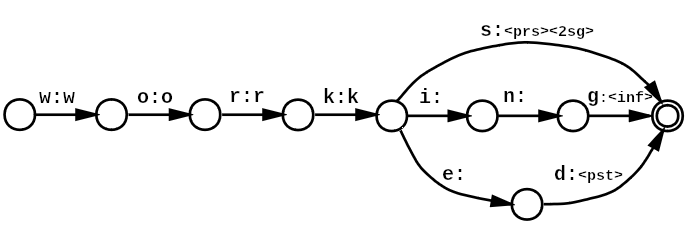
\includegraphics[scale=0.5]{\rootdir/img/transducer1_1.png}
    \caption{A modified version of Figure \ref{fig:fst1} which takes as input \textit{works}, \textit{working}, \textit{worked} and outputs \textit{work<prs><2sg>}, \textit{work<inf>}, \textit{work<pst>} respectively.}
    \label{fig:fst1_1}
\end{figure}

\subsubsection{FST formalisms}
By FST formalism I mean a human-readable formal language that can be compiled into a static FST, or from what a FST behavior can be emulated in runtime. A FST formalism usually includes a way to list lexicons and/or list lexicon combination rules and/or list phonological rules.

One of the first major fundamental advances was when \parencite{koskenniemi_twol_1983} created a model, which introduced a FST formalism named Two-level morphology (TWOL) for describing morphological and morphonological paradigms. Its novice was in the addition of the phonology level of rules, which made it much easier and intuitive to implement cases like \textit{`eye(-s)'/`box(-es)'}. This model was capable of word-form recognition and production, but it was not yet compilable into static FSTs, it was working at runtime and was known for being slow. Then \textcite{karttunen_twolc_1987} at Xerox Research Center developed a Two-level rule Compiler (\texttt{twolc}), which compiled TWOL rules into static FSTs. Later a separate compiler for lexicon definitions was introduced named \texttt{lexc} (\textbf{Lex}icon \textbf{C}ompiler) \parencite{karttunen_lexc_1993}, it came with its own formalism language for describing lexicon and morphotactics. The standard approach to modeling a language at that point was using \texttt{lexc} to describe lexicon and morphology and \texttt{twolc} to describe morphonology, which stayed almost the same to this day. 

One of the latest released tools was \texttt{lexd} lexicon compiler \parencite{swanson_lexd_2021}. It is presented as a \texttt{lexc} alternative and is  claimed to be much faster in the compilation time. It also introduced a tag system, which allows FST developers to specify how diffetent lexicons combine with each other more precisely. \todo{anything else?}

\todo{Есть еще апертиумовский lttoolbox, так что Вам возможно стоит мотивировать, почему Вы его не используете.}

\subsubsection{Helsinki finite-state technology}
Helsinki finite-state technology (HFST) is a set of tools for creating and working with languages' morphology models in form of transducers \parencite{linden_hfst_2009}. It includes implementations of both \texttt{hfst-lexc} and \texttt{hfst-twolc} compilers, as well as command line interface commands for mathematical and other miscellaneous operations with transducers like FST combination and format conversion. Also, it comes with a file format \texttt{.hfst} designed to store compiled FSTs.

HFST is widely applied when it comes to creating rule-based morphological models. Some of the latest examples of HFST-based morphological tools are: morphological parser for the Tamil language by \textcite{sarveswaran_morph_2021}, a morphological transducer for Kyrgyz by \textcite{washington_finite_2012}, a morphological parser for Andi by \textcite{buntyakova_2023_twol} and a morphological parser for the Chamalal language by \textcite{budilova_2023_twol}.

\todo{Раз уж Вы здесь добавляете ссылки, я бы сослался на Даню Игнатьева и багвалинский. https://github.com/ruthenian8/bagvalal}

\subsection{Existing morphology models for Shughni}
At this time only one morphological parser exists for Shughni. It was developed by \textcite{melenchenko_2021_parser} and was later included in `Digital Resources for the Shughni Language' project \parencite{makarov_digital_2022}. It is a rule-based parser implemented in Python which shows good coverage and accuracy results. The main difference from the parser presented in this work is that Melenchenko's parser is not based on FST technology.

\todo{Опять эта же проблема. Мне не кажется, что если что-то не сделано в FST, сразу надо делать FST аналог. В данном разделе следует подробнее описать преимущества и недостатки парсера Максима.}